\documentclass{article}
\usepackage{graphicx} 
\usepackage{cite}
\usepackage{amsmath,amssymb,amsfonts}
\usepackage{algorithmic}
\usepackage{textcomp}
\usepackage{xcolor}
\usepackage{booktabs}
\usepackage{arydshln}
\usepackage[a4paper, margin=1in]{geometry}
\usepackage{algorithm}
\usepackage{algorithmic}
\usepackage{placeins}
\usepackage{float}

\title{Laboratory 3}
\author{Víctor Brull Rico\and
        Guillem Martínez Sambola}
\date{May 14, 2026}

\begin{document}

\maketitle

\section{Introduction}



\section{Methods}
\label{sec:Methods}

\subsection{Texture Synthesis by Non-parametric Sampling}

The non-parametric sampling method for texture synthesis, introduced by Efros and Leung~\cite{efros1999}, models texture as a Markov Random Field (MRF). In this model, each pixel $p$ is assumed to be conditionally independent of all other pixels in the image, given its local neighborhood window $\omega(p)$ of size $w \times w$. This locality assumption allows the synthesis process to focus only on the spatial context around each pixel.

The synthesis procedure begins with a small seed region, typically a $3 \times 3$ patch, randomly sampled from the input texture. The algorithm then grows the synthesized image outward, layer by layer, filling in one pixel at a time along the current boundary of known pixels. For each pixel to be synthesized, the algorithm:
\begin{enumerate}
    \item Extracts the known neighborhood $\omega(p)$ around the pixel.
    \item Searches the sample image for all patches whose known neighborhoods are similar to $\omega(p)$, using a Gaussian-weighted sum of squared differences (SSD) as the similarity metric.
    \item Selects all candidate patches whose SSD is within a tolerance $\epsilon$ of the best (minimum) SSD found.
    \item Randomly chooses one of these candidates and copies its center pixel value to the synthesized image.
\end{enumerate}

The Gaussian-weighted SSD distance is defined as:
\begin{equation}
    d(\omega_1, \omega_2) = \sum_{i} G_i \cdot ({\omega_1}_i - {\omega_2}_i)^2,
    \label{eq:ssd}
\end{equation}
where $G$ is a 2D isotropic Gaussian kernel centered in the window, giving more importance to pixels near the center of the neighborhood. This weighting helps preserve local structure and reduces the influence of less relevant, distant pixels.

The tolerance parameter $\epsilon$ controls the diversity of the synthesis: a larger $\epsilon$ allows more candidate patches to be considered, resulting in more stochastic and varied outputs, while a smaller $\epsilon$ makes the synthesis more deterministic and faithful to the input texture.

When computing the SSD, only the known (already synthesized) pixels in the window are used; unknown pixels are ignored. The SSD is normalized by the total weight of the known pixels, ensuring that distances are comparable even when the number of known neighbors varies.

The patch window size $w$ is a key free parameter of the method, as it determines the size of the local context used for matching and synthesis. Larger windows capture more structure but require more computation and may reduce the diversity of the output.

The method of Efros and Leung~\cite{efros1999} models texture as a Markov
Random Field. A pixel $p$ is assumed to be conditionally independent of the
rest of the image given its square neighborhood window $\omega(p)$ of width
$w$. Texture is synthesized by growing outward from a small seed, one pixel
at a time. For each candidate pixel, all neighborhoods in the sample image
that are similar to $\omega(p)$ are found using a Gaussian-weighted sum of
squared differences (SSD):
\begin{equation}
    d(\omega_1, \omega_2) = \sum_{i} G_i \cdot ({\omega_1}_i - {\omega_2}_i)^2,
    \label{eq:ssd}
\end{equation}
where $G$ is a 2D isotropic Gaussian kernel that gives more weight to pixels
near the center. Unknown (not yet synthesized) pixels are excluded from the
sum, and the result is normalized by the total weight of the known pixels.
All patches $\omega$ satisfying
$d(\omega(p), \omega) < (1+\epsilon)\,d(\omega(p), \omega_{\text{best}})$
are considered valid candidates, and a random one is selected.

\subsection{Implementation Details}

The implementation is modular, with two core functions supporting the synthesis process:

\texttt{extract\_patches.m} extracts all possible $w \times w$ patches from the sample image. It slides a window over the image, collecting only those patches whose support lies entirely within the image boundaries (i.e., the window does not extend beyond the image edges). Each patch is stored as a column in a 4D array of size $(w, w, C, N)$, where $C$ is the number of color channels and $N$ is the total number of patches. The function also returns the coordinates of the patch centers, maintaining the same order as the patches in the array.

\texttt{compute\_patch\_distances.m} computes the Gaussian-weighted SSD between a query patch and all patches in the list. It applies a binary mask to indicate which pixels in the query patch are known (already synthesized), and multiplies this mask with the Gaussian weights to form a combined weight map. The SSD is then computed only over the known pixels, and the result is normalized by the sum of the weights for those pixels. This ensures that the distance is meaningful even when some pixels are unknown. The function is fully vectorized: it computes the distances between the query patch and all patches in the list simultaneously, leveraging MATLAB's array operations for efficiency. This vectorization significantly speeds up the computation compared to a naive loop over patches.

The following pseudocode summarizes the patch extraction and distance computation:
\begin{verbatim}
% Patch extraction
for each valid center (r, c) in image:
    patch = image(r-half_h:r+half_h, c-half_w:c+half_w, :)
    store patch and (r, c)

% Patch distance computation
for each patch in patch_list:
    diff = patch - query_patch
    weighted_sq = (diff.^2) .* combined_weights
    distance = sum(weighted_sq) / sum(combined_weights)
\end{verbatim}

By organizing the code in this way, the method efficiently supports the non-parametric sampling approach for texture synthesis.

We implemented two core functions. \texttt{extract\_patches} slides a
$w \times w$ window over the sample image and stores each valid patch
(whose support lies entirely within the image) as a column of a matrix of
size $(w^2 \cdot C) \times N$, where $C$ is the number of channels and $N$
is the number of patches. \texttt{compute\_patch\_distances} computes the
Gaussian-weighted SSD between a query patch and all columns of this matrix,
masking out unknown pixels and normalizing by the total weight of known ones.
Vectorizing the distance computation over all patches simultaneously gave a
significant speedup compared to iterating patch by patch.


\section{Experiments}
\label{sec:Experiments}

\subsection{Testing Texture Synthesis}

Bricks example. Sample images:

\begin{figure}[H]
\centering
\resizebox{\linewidth}{!}{
\begin{tabular}{@{}cc@{}}
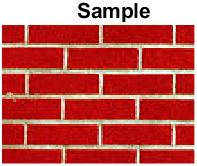
\includegraphics[width=0.5\linewidth]{Figures/bricks_sample.png} &
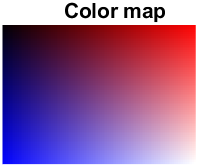
\includegraphics[width=0.5\linewidth]{Figures/bricks_color_map.png} \\
\small Sample & \small Color Map \\
\end{tabular}}
\caption{Sample and color map for the bricks example.}
\label{fig:bricks-sample}
\end{figure}

Vary patch size, keep tolerance fixed. Texture and copy map for patch_size = 5, 11, 23, 31 and tolerance = 0.1:

\begin{figure}[H]
\centering
\resizebox{\linewidth}{!}{
\begin{tabular}{@{}cc@{}}
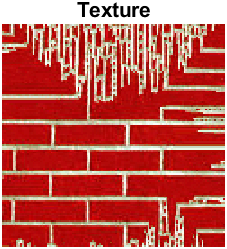
\includegraphics[width=0.5\linewidth]{Figures/bricks_text_5_01.png} &
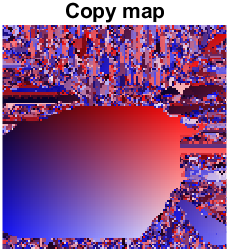
\includegraphics[width=0.5\linewidth]{Figures/bricks_cm_5_01.png} \\
\small Texture & \small Copy Map \\
\end{tabular}}
\caption{Small patch. Texture and copy map for patch_size = 5 and tolerance = 0.1.}
\label{fig:bricks-results-5-01}
\end{figure}

\begin{figure}[H]
\centering
\resizebox{\linewidth}{!}{
\begin{tabular}{@{}cc@{}}
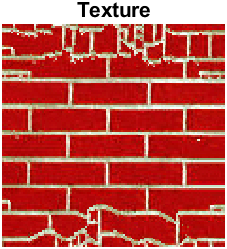
\includegraphics[width=0.5\linewidth]{Figures/bricks_text_11_01.png} &
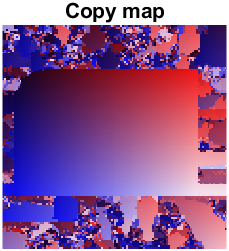
\includegraphics[width=0.5\linewidth]{Figures/bricks_cm_11_01.png} \\
\small Texture & \small Copy Map \\
\end{tabular}}
\caption{Medium patch. Texture and copy map for patch_size = 11 and tolerance = 0.1.}
\label{fig:bricks-results-11-01}
\end{figure}

\begin{figure}[H]
\centering
\resizebox{\linewidth}{!}{
\begin{tabular}{@{}cc@{}}
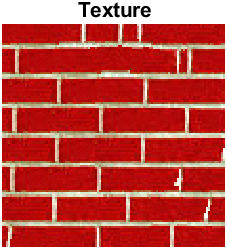
\includegraphics[width=0.5\linewidth]{Figures/bricks_text_23_01.png} &
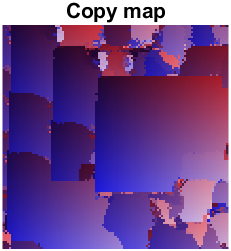
\includegraphics[width=0.5\linewidth]{Figures/bricks_cm_23_01.png} \\
\small Texture & \small Copy Map \\
\end{tabular}}
\caption{Large patch. Texture and copy map for patch_size = 23 and tolerance = 0.1.}
\label{fig:bricks-results-23-01}
\end{figure}

\begin{figure}[H]
\centering
\resizebox{\linewidth}{!}{
\begin{tabular}{@{}cc@{}}
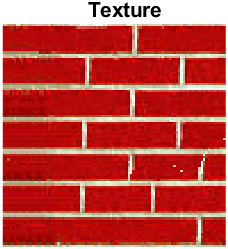
\includegraphics[width=0.5\linewidth]{Figures/bricks_text_31_01.png} &
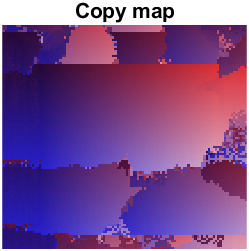
\includegraphics[width=0.5\linewidth]{Figures/bricks_cm_31_01.png} \\
\small Texture & \small Copy Map \\
\end{tabular}}
\caption{Extreme large patch. Texture and copy map for patch_size = 31 and tolerance = 0.1.}
\label{fig:bricks-results-31-01}
\end{figure}

Vary tolerance, keep patch size fixed. Texture and copy map for patch_size = 23 and tolerance = 0.01, 0.1, 1.0.
Keep patch_size = 23 given the results above, as it provides the best balance.

\begin{figure}[H]
\centering
\resizebox{\linewidth}{!}{
\begin{tabular}{@{}cc@{}}
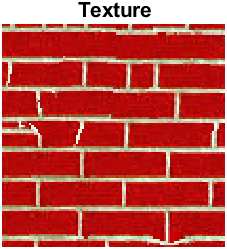
\includegraphics[width=0.5\linewidth]{Figures/bricks_text_23_001.png} &
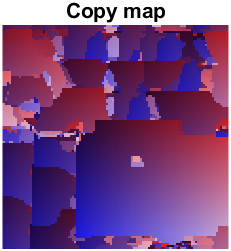
\includegraphics[width=0.5\linewidth]{Figures/bricks_cm_23_001.png} \\
\small Texture & \small Copy Map \\
\end{tabular}}
\caption{Low tolerance. Texture and copy map for patch_size = 23 and tolerance = 0.01.}
\label{fig:bricks-results-23-001}
\end{figure}

\begin{figure}[H]
\centering
\resizebox{\linewidth}{!}{
\begin{tabular}{@{}cc@{}}
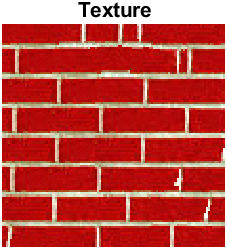
\includegraphics[width=0.5\linewidth]{Figures/bricks_text_23_01.png} &
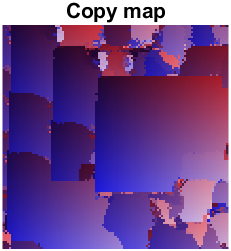
\includegraphics[width=0.5\linewidth]{Figures/bricks_cm_23_01.png} \\
\small Texture & \small Copy Map \\
\end{tabular}}
\caption{Medium tolerance. Texture and copy map for patch_size = 23 and tolerance = 0.1.}
\label{fig:bricks-results-23-01}
\end{figure}

\begin{figure}[H]
\centering
\resizebox{\linewidth}{!}{
\begin{tabular}{@{}cc@{}}
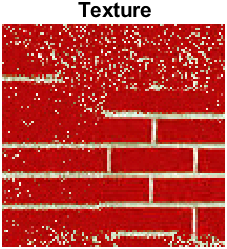
\includegraphics[width=0.5\linewidth]{Figures/bricks_text_23_1.png} &
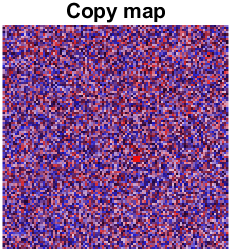
\includegraphics[width=0.5\linewidth]{Figures/bricks_cm_23_1.png} \\
\small Texture & \small Copy Map \\
\end{tabular}}
\caption{High tolerance. Texture and copy map for patch_size = 23 and tolerance = 1.0.}
\label{fig:bricks-results-23-10}
\end{figure}

Cells example. Sample images:

\begin{figure}[H]
\centering
\resizebox{\linewidth}{!}{
\begin{tabular}{@{}cc@{}}
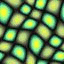
\includegraphics[width=0.5\linewidth]{Figures/cells_sample.png} &
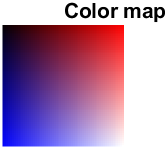
\includegraphics[width=0.5\linewidth]{Figures/cells_color_map.png} \\
\small Sample & \small Color Map \\
\end{tabular}}
\caption{Sample and color map for the cells example.}
\label{fig:cells-sample}
\end{figure}

Vary patch size, keep tolerance fixed. Texture and copy map for patch_size = 5, 11, 23, 31 and tolerance = 0.1:

\begin{figure}[H]
\centering
\resizebox{\linewidth}{!}{
\begin{tabular}{@{}cc@{}}
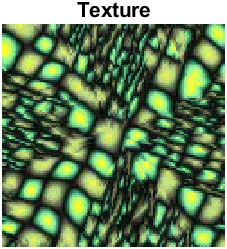
\includegraphics[width=0.5\linewidth]{Figures/cells_text_5_01.png} &
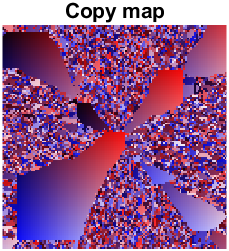
\includegraphics[width=0.5\linewidth]{Figures/cells_cm_5_01.png} \\
\small Texture & \small Copy Map \\
\end{tabular}}
\caption{Small patch. Texture and copy map for patch_size = 5 and tolerance = 0.1.}
\label{fig:cells-results-5-01}
\end{figure}

\begin{figure}[H]
\centering
\resizebox{\linewidth}{!}{
\begin{tabular}{@{}cc@{}}
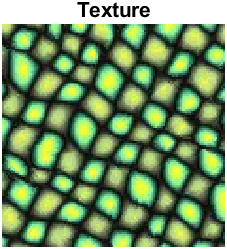
\includegraphics[width=0.5\linewidth]{Figures/cells_text_11_01.png} &
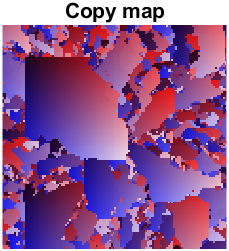
\includegraphics[width=0.5\linewidth]{Figures/cells_cm_11_01.png} \\
\small Texture & \small Copy Map \\
\end{tabular}}
\caption{Medium patch. Texture and copy map for patch_size = 11 and tolerance = 0.1.}
\label{fig:cells-results-11-01}
\end{figure}

\begin{figure}[H]
\centering
\resizebox{\linewidth}{!}{
\begin{tabular}{@{}cc@{}}
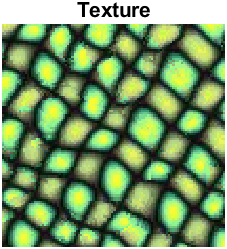
\includegraphics[width=0.5\linewidth]{Figures/cells_text_23_01.png} &
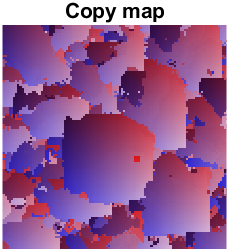
\includegraphics[width=0.5\linewidth]{Figures/cells_cm_23_01.png} \\
\small Texture & \small Copy Map \\
\end{tabular}}
\caption{Large patch. Texture and copy map for patch_size = 23 and tolerance = 0.1.}
\label{fig:cells-results-23-01}
\end{figure}

\begin{figure}[H]
\centering
\resizebox{\linewidth}{!}{
\begin{tabular}{@{}cc@{}}
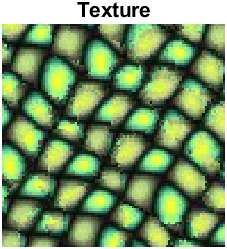
\includegraphics[width=0.5\linewidth]{Figures/cells_text_31_01.png} &
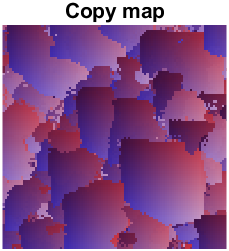
\includegraphics[width=0.5\linewidth]{Figures/cells_cm_31_01.png} \\
\small Texture & \small Copy Map \\
\end{tabular}}
\caption{Extreme large patch. Texture and copy map for patch_size = 31 and tolerance = 0.1.}
\label{fig:cells-results-31-01}
\end{figure}

Vary tolerance, keep patch size fixed. Texture and copy map for patch_size = 23 and tolerance = 0.01, 0.1, 1.0.
Keep patch_size = 23 given the results above, as it provides the best balance.

\begin{figure}[H]
\centering
\resizebox{\linewidth}{!}{
\begin{tabular}{@{}cc@{}}
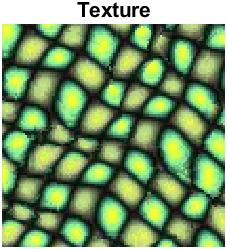
\includegraphics[width=0.5\linewidth]{Figures/cells_text_23_001.png} &
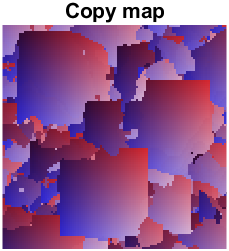
\includegraphics[width=0.5\linewidth]{Figures/cells_cm_23_001.png} \\
\small Texture & \small Copy Map \\
\end{tabular}}
\caption{Low tolerance. Texture and copy map for patch_size = 23 and tolerance = 0.01.}
\label{fig:cells-results-23-001}
\end{figure}

\begin{figure}[H]
\centering
\resizebox{\linewidth}{!}{
\begin{tabular}{@{}cc@{}}
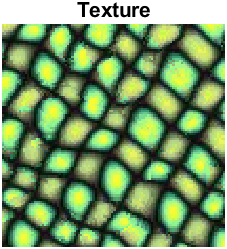
\includegraphics[width=0.5\linewidth]{Figures/cells_text_23_01.png} &
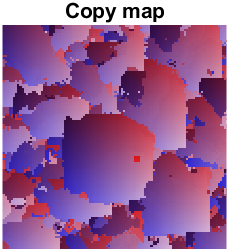
\includegraphics[width=0.5\linewidth]{Figures/cells_cm_23_01.png} \\
\small Texture & \small Copy Map \\
\end{tabular}}
\caption{Medium tolerance. Texture and copy map for patch_size = 23 and tolerance = 0.1.}
\label{fig:cells-results-23-01}
\end{figure}

\begin{figure}[H]
\centering
\resizebox{\linewidth}{!}{
\begin{tabular}{@{}cc@{}}
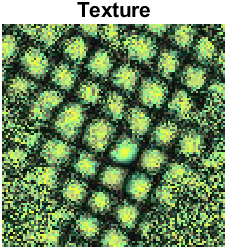
\includegraphics[width=0.5\linewidth]{Figures/cells_text_23_1.png} &
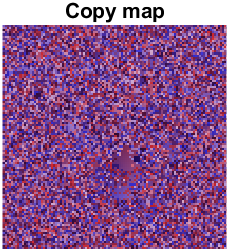
\includegraphics[width=0.5\linewidth]{Figures/cells_cm_23_1.png} \\
\small Texture & \small Copy Map \\
\end{tabular}}
\caption{High tolerance. Texture and copy map for patch_size = 23 and tolerance = 1.0.}
\label{fig:cells-results-23-10}
\end{figure}



\section{Conclusion}
\label{sec:Conclusion}




\bibliographystyle{IEEEbib}
\bibliography{references}

\end{document}
